\documentclass[border=3pt,tikz]{standalone}
\usetikzlibrary{arrows}
\usetikzlibrary{positioning}
\usetikzlibrary{calc}
\usetikzlibrary{arrows}
\begin{document}
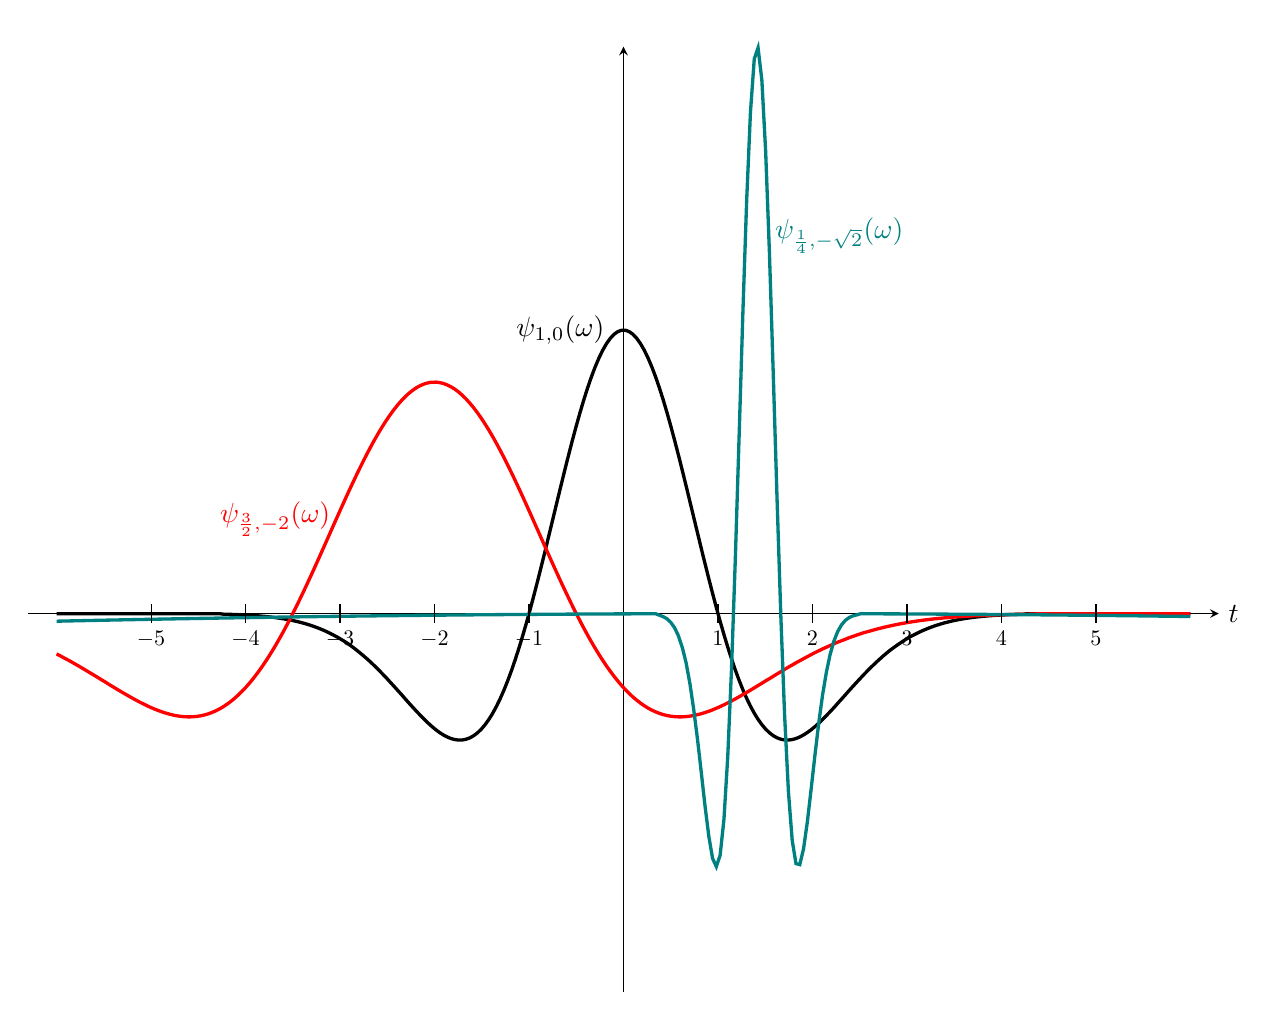
\begin{tikzpicture}[samples = 200, scale=1.2]

\draw[-{stealth}] (-6.3, 0) -- (6.3,0) node[right] {$t$};
\draw[-{stealth}] (0,-4) -- (0,6) node[above] {$$};
\draw[color=black, very thick, domain=-6:6, samples=300, variable = \t]   plot ({\t}, {3*(1-(\t)^2)*exp(-\t*\t/2)});
\draw[color=red, very thick, domain=-6:6, samples=300, variable = \t]   plot ({\t}, { 3*sqrt(2)/sqrt(3) * (1-((\t+2)/1.5)^2)*exp(-(((\t+2)/1.5)^2)/2)});

\draw[color=teal, very thick, domain=-6:6, samples=300, variable = \t]   plot ({\t}, { 3*sqrt(4)* (1-((\t-sqrt(2))*4)^2)*exp(-(((\t-sqrt(2))*4)^2)/2)});

\node [left] at (-0.1, 3) {$\psi_{1, 0}(\omega)$};
\node [left, red] at (-3, 1) {$\psi_{\frac{3}{2}, -2}(\omega)$};
\node [right, teal] at (1.5, 4) {$\psi_{\frac{1}{4}, -\sqrt{2}}(\omega)$};

\foreach \x in {1,...,5}
{
    \draw (\x, 0.1)-- (\x, -0.1) node[below, scale=0.8] {$\x$};
    \draw (-\x, 0.1)-- (-\x, -0.1) node[below, scale=0.8] {$-\x$};
}

\end{tikzpicture}
\end{document}